%!TEX TS-program = xelatex
\documentclass[]{friggeri-cv}
\usepackage{afterpage}
\usepackage{hyperref}
\usepackage{color}
\usepackage{xcolor}
\usepackage{smartdiagram}
\usepackage{fontspec}
% if you want to add fontawesome package
% you need to compile the tex file with LuaLaTeX
% References:
%   http://texdoc.net/texmf-dist/doc/latex/fontawesome/fontawesome.pdf
%   https://www.ctan.org/tex-archive/fonts/fontawesome?lang=en
% \usepackage{fontawesome}
\usepackage{metalogo}
% \usepackage{dtk-logos}
\usepackage[utf8]{inputenc}
\usepackage{tikz}
\usetikzlibrary{mindmap,shadows}
\hypersetup{
    pdftitle={},
    pdfauthor={},
    pdfsubject={},
    pdfkeywords={},
    colorlinks=false,           % no lik border color
    allbordercolors=white       % white border color for all
}
\smartdiagramset{
    bubble center node font = \footnotesize,
    bubble node font = \footnotesize,
    % specifies the minimum size of the bubble center node
    bubble center node size = 0.5cm,
    %  specifies the minimum size of the bubbles
    bubble node size = 0.5cm,
    % specifies which is the distance among the bubble center node and the other bubbles
    distance center/other bubbles = 0.3cm,
    % sets the distance from the text to the border of the bubble center node
    distance text center bubble = 0.5cm,
    % set center bubble color
    bubble center node color = pblue,
    % define the list of colors usable in the diagram
    set color list = {lightgray, materialcyan, orange, green, materialorange, materialteal, materialamber, materialindigo, materialgreen, materiallime},
    % sets the opacity at which the bubbles are shown
    bubble fill opacity = 0.6,
    % sets the opacity at which the bubble text is shown
    bubble text opacity = 0.5,
}

\addbibresource{bibliography.bib}
\RequirePackage{xcolor}
\definecolor{pblue}{HTML}{0395DE}

\begin{document}
\header{Mathieu}{Neron}
      {Software Engineer}
      
% Fake text to add separator      
\fcolorbox{white}{gray}{\parbox{\dimexpr\textwidth-2\fboxsep-2\fboxrule}{%
.....
}}

% In the aside, each new line forces a line break
\begin{aside}
  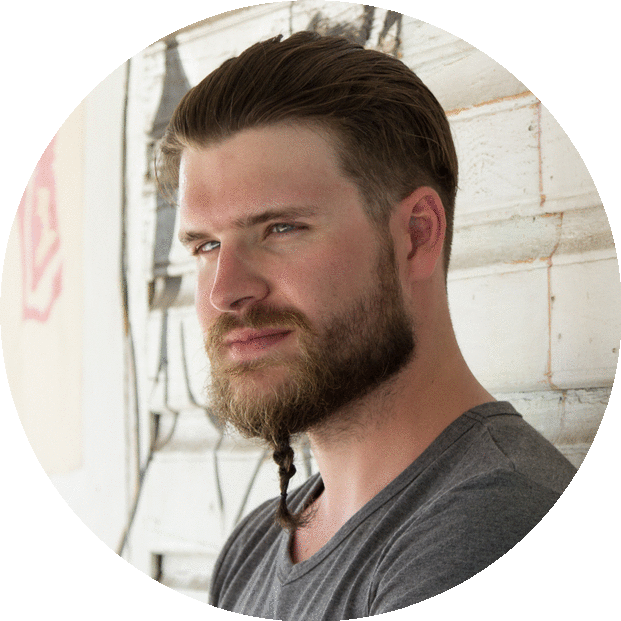
\includegraphics[scale=0.18]{img/mathieu.png}
  \section{Address}
    1032 Mississippi Street
    San Francisco, CA
    94107
    United States
    ~
  \section{Tel}
    628-358-8813
    ~
  \section{Mail}
    \href{mailto:mathieu.neron.ing@gmail.com}{\textbf{mathieu.neron.ing@}\\gmail.com}
    ~
  \section{Web \& Git}
    \href{https://ca.linkedin.com/in/mathieu-n\%C3\%A9ron-b4419522}{Linkedin profile}
\href{https://github.com/mathieu-neron}{Github account}
    ~
  % use  \hspace{} or \vspace{} to change bubble size, if needed
  \section{Programming}
    \smartdiagram[bubble diagram]{
        \textbf{Java},
        \textbf{Matlab},
        \textbf{C/C++},
        \textbf{Bash},
        \textbf{React},
        \textbf{Angular},
        \textbf{JS/Typescript},
        \textbf{HTML/CSS},
        \textbf{C\#/.NET}
    }
    ~
  \section{Personal Skills}
    \smartdiagram[bubble diagram]{
        \textbf{Team}\\\textbf{Player},
        \textbf{Initiative},
        \textbf{Curiosity},
        \textbf{Problem}\\\textbf{Solving},
        \textbf{\vspace{2mm}Learn/Teach\vspace{2mm}},
        \textbf{Organize}
    }
    ~
\end{aside}
~
\section{Summary}

Software engineer with over 12 years of accumulated professional/internship experience. Versatile, bilingual professional with expertise from projects in the aerospace, gaming, consulting, e-signature, finance and data visualization industry.
\section{Experience}
\begin{entrylist}
%------------------------------------------------

\entry
{2018--Now}
{Tableau}
{Paleau Alto, United States}
{\emph{Senior Software Developer -> LMTS} (React, Typescript, Java, C#, Qt, C++)
\begin{itemize}
	\item \textbf{Improved} upon the newly released Object Graph project in the Data pane of Tableau, by adding transition animations, updated tooltips, alphabetical sorting in the graph, implemented rerooting, etc.
	\item \textbf{Contributed} to the hybridization of a new Data Preview Area module to showcase the metadata/data grid + embedded relationship editor. 
	\item \textbf{Onboarded} a new AI predictive model content type within Tableau Server, in order to support a Salesforce integration with Einstein.
	\item \textbf{Participated} in a few recruiting interviews and mentored an intern during the summer of 2021, alongside one of my colleague.
\end{itemize}
}

%------------------------------------------------

\entry
{2016--2018}
{Paysafe}
{Montréal, Canada}
{\emph{Java Developer} (Angular 2+, Typescript, Java 7/8, Spring, Oracle)
\begin{itemize}
	\item \textbf{Trailblazed} on a new frontend project in Angular 2+ for the new Merchant Portal application.
	\item \textbf{Invigorated} the Netbanx codebase by fixing bugs, adding unit tests. removing errors/warnings and implementing new features.
	\item \textbf{Slashed} execution time of frontend tests by a factor of six by switching from PhantomJs to the Nightmage browser automation library.
\end{itemize}
}

%------------------------------------------------

\entry
{2014--2016}
{eSignLive by Vasco}
{Montréal, Canada}
{\emph{Java Developer} (Java 7/8, Guava, Spring, AWS, MySQL)
\begin{itemize}
\item \textbf{Implemented and took ownership} of features requested by the product manager that were integrated in the eSignLive core application, processing over a billion documents/signatures each year.
\item \textbf{Fixed} bugs in the backend codebase. Added API tests, increased code coverage by over 85\% on classes with unit tests and applied the campfire rule when possible to insure quality and maintainability.
\item \textbf{Reduced} downtime of the Windows document converter by 50\%.
\item \textbf{Integrated} technologies: Equifax, Twilio, PDFBox, Google Noto Fonts.
\item \textbf{Supported} other team members by reducing their time spent investigating for a solution by providing my support and insight whenever needed. Also showcased the backend architecture to multiple new hires.
\end{itemize}
}

%------------------------------------------------

\entry
{2012--2014}
{Avanade}
{Montréal, Canada}
{\emph{Application Developer:}
\textbf{Consulted} on the following contracts:
\begin{itemize}
\item \emph{CN (C\#/.NET, Sitecore)}
\begin{itemize}
	\item \textbf{Redesigned} the www.cn.ca website with other Avanade developers using Sitecore and C\#/.NET, the main menu being my biggest contribution.
\end{itemize}
\item \emph{Hydro-Québec (Javascript, SAPUI5, Infragistics)}
\begin{itemize}
	\item \textbf{Programmed} an internal web-based time spreadsheet application used by Hydro-Quebec managers on their various projects.
\end{itemize}
\end{itemize}
}
\end{entrylist}

\newpage

\begin{aside}
~
~
~
  \section{OS Preference}
    \textbf{GNU/Linux}
\includegraphics[scale=0.40]{img/5stars.png}
    \textbf{MacOS}
\includegraphics[scale=0.40]{img/4stars.png}
    \textbf{Windows}
\includegraphics[scale=0.40]{img/3stars.png}
    ~
  \section{Languages}
    \textbf{French}
\includegraphics[scale=0.40]{img/5stars.png}
    \textbf{English}
\includegraphics[scale=0.40]{img/4stars.png}
    ~
\end{aside}

%----------------------------------------------------------------------------------------
%	INTERNSHIP EXPERIENCE SECTION
%----------------------------------------------------------------------------------------

\section{Internship Experience}

\begin{entrylist}

\entry
{2011}
{Electronic Arts Canada}
{Burnaby, Canada}
{\emph{Software Engineer Intern} (C\#/.NET, C++)
	\begin{itemize}
		\item \textbf{Implemented} a distributed system in C++/C\# managing thousands of simultaneous automated online bots to test the load on SSX snowboard game's server, in collaboration with the Online/UI team.
		\item \textbf{Designed and assembled} a telemetry lookup system in ASP.NET using heat map data to illustrate the activity of players.
		\item \textbf{Showcased} the online bot tool to fellow interns, which was used afterwards to help present the multiplayer component of the game at Gamescom in Germany.
	\end{itemize}}

%------------------------------------------------

\entry
{2010}
{Autodesk}
{Montréal, Canada}
{\emph{Software Engineer Intern} (C++, Qt, Python)
\begin{itemize}
	\item \textbf{Developed} an animation plug-in inside the Maya software using C++ and Qt with 4 other members of the Games team.
	\item \textbf{Wrote and tested} mathematical functions in Python for a bloc programming tool used by designers/artists for animation blending, applying what I learned during the internship.
\end{itemize}}

%------------------------------------------------

\entry
{2009}
{Ubisoft}
{Québec, Canada}
{\emph{QA Developer Intern} (C\#/.NET)
\begin{itemize}
	\item \textbf{Developed/expanded} C\# tools which were used by the dev teams of the studio to improve performance/conviviality.
	\item \textbf{Maintained and provided} support for the tool suite developed by correcting any bug that would arise.
\end{itemize}}

%------------------------------------------------

\entry
{2008}
{Lockheed Martin}
{Montréal, Canada}
{\emph{Software Evaluator Intern}
	\begin{itemize}
		\item \textbf{Evaluated} a simulation software and insured its quality by writing automated test in Javascript with the TestComplete IDE in addition to writing procedure documentation.
		\item \textbf{Presented} the product in Halifax to clients and helped them understand its inner workings by providing a crash course as well.
	\end{itemize}}

%------------------------------------------------

\end{entrylist}

\section{Education}
\begin{entrylist}
    \entry
{2007--2011}
{Bachelor {\normalfont of Computer Engineering}}
{Université de Sherbrooke}
{Specialization in Software Engineering \& Artificial Intelligence}
\end{entrylist}

%----------------------------------------------------------------------------------------
%	CERTIFICATIONS \& CONFERENCES SECTION
%----------------------------------------------------------------------------------------

\section{Certifications \& Conferences}

\begin{itemize}
	\item Sharepoint 2010 Boot Camp
	\item Consulting Excellence Foundations (April 2013)
	\item Codility Certification: \href{https://codility.com/cert/view/cert6AG9RU-X7CHVB5QVHFTSAZ4/}{https://codility.com/cert/view/cert6AG9RU-X7CHVB5QVHFTSAZ4/}
	\item Angular 2 Professional Certification (December 2016)
	\item QCon New York 2018 Conference
	\item Tableau 2018 Boot Camp
\end{itemize}

\newpage

%----------------------------------------------------------------------------------------
%	INTERESTS SECTION
%----------------------------------------------------------------------------------------

\section{Interests}

\textbf{Professional:} cryptocurrency (did some mining back in 2013-2014), functional programming, machine learning \& data science, software architecture, algorithms, design patterns, agile methodologies.
\\
\textbf{Personal:} saxophone, reading, cooking, skiing, running, biking, hiking, traveling
\\
\begin{flushleft}
\emph{February 19th, 2021}
\end{flushleft}
\begin{flushright}
\emph{Mathieu Neron}
\end{flushright}

\end{document}
